\chapter{Analytical techniques and tools} \label{chap4}

The parts that follow go over the most important analysis and approaches for studying, modeling, and predicting ECG arrhythmia diagnosis.

\section{Commonly used techniques and tools} \label{4commontools}

\subsection{Data Wrangling (DW)} \label{4dw}

Data wrangling is the act of cleaning and combining chaotic and difficult data sets for easy access and analysis. With the amount of data and data sources growing all the time, it's more vital than ever to arrange massive volumes of data for analysis \cite{datawrang}. To facilitate data consumption and organization, this method normally requires manually transforming and mapping data from one raw format to another.

The most relevant Data Wrangling's objectives are \cite{datawrang}:

\begin{itemize}
    \item Collect data from a variety of sources in order to uncover "deeper intelligence."
    \item As soon as feasible, get reliable, actionable data into the hands of business analysts.
    \item Reduce the amount of time it takes to collect and organize jumbled data before it can be used.
    \item Allow data scientists and analysts to focus on data analysis instead of data manipulation.
    \item Encourage senior executives in a company to improve their decision-making skills.
\end{itemize}

\begin{figure}[H]
\centering
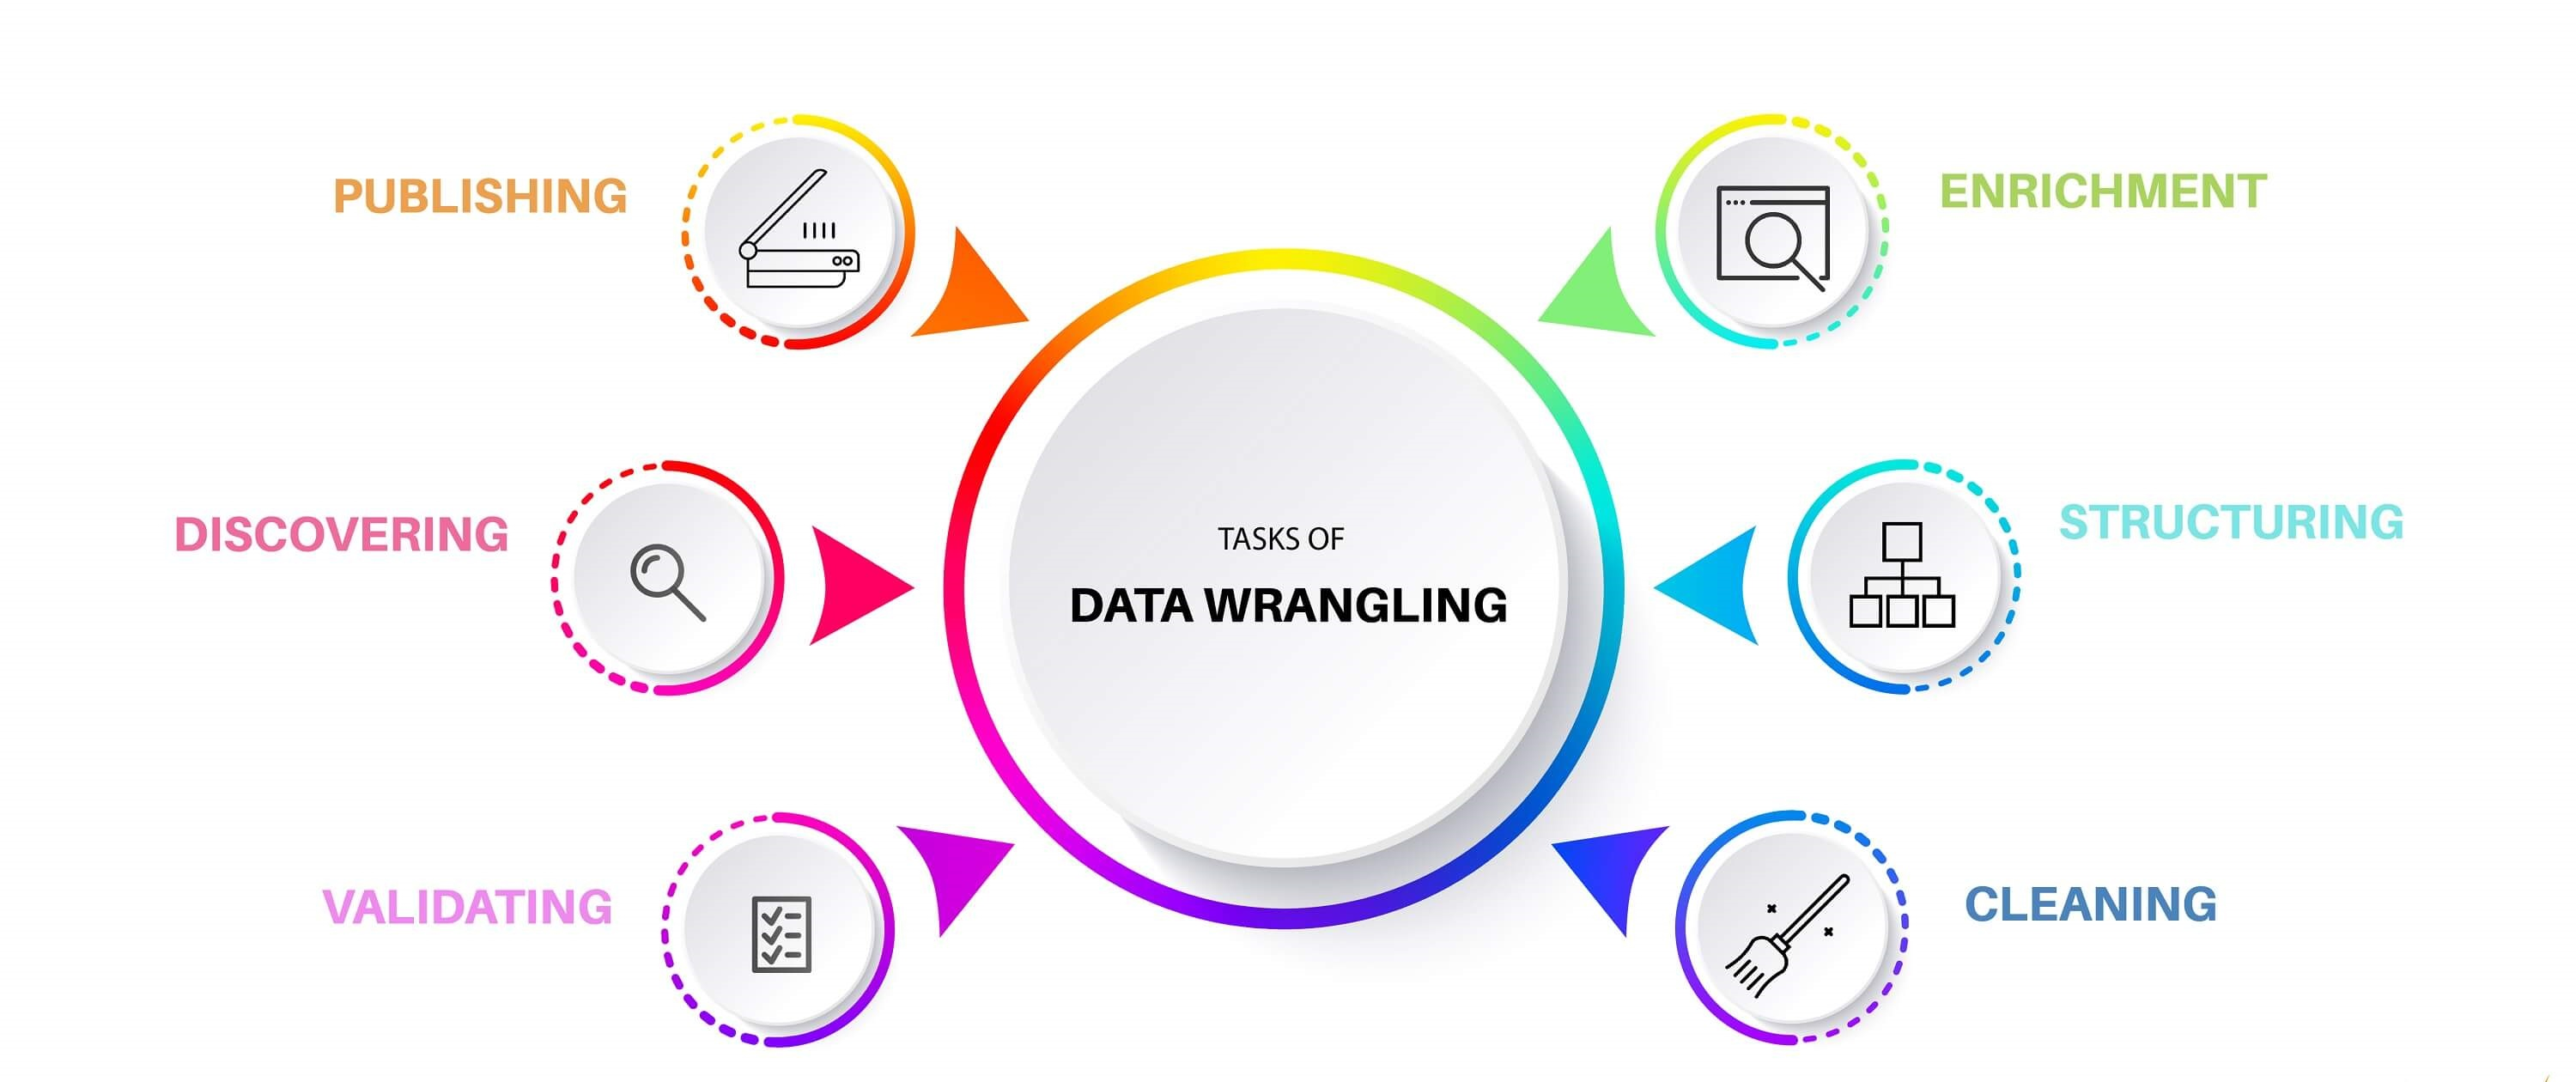
\includegraphics[scale=0.18]{img/DATA_WRANGLING.jpg}
\caption{Main steps in Data Wrangling}
\label{fig:dwprocess}
\end{figure}

The data wrangling approach typically consists of six iterative steps, as seen in Figure \ref{fig:dwprocess}, as mentioned by \cite{datawrang2}:

\begin{enumerate}
    \item \textbf{Publishing:} Data wranglers prepare data for downstream usage - whether by a specific user or program - and identify any special actions or logic that were employed to do so. 
    
    \item \textbf{Discovering:} Before delving into the data, it's important to first have a better knowledge of what's there, since this will influence how you examine the data.

    \item \textbf{Validating:} These are recurrent programming sequences that verify data quality, consistency, and security. Validation can include things like ensuring that qualities that should be distributed on a regular basis are distributed uniformly.
    
    \item \textbf{Enrichment:} "What more types of data can be obtained from what already exists?" one can question during the data wrangling stage. or "What further information could assist me in making better selections based on the current data?"
    
    \item \textbf{Structuring:} The data must be structured in this step of data wrangling because raw data arrives in a range of formats and sizes.
    
    \item \textbf{Cleaning:} By altering null values and establishing standard formats, data wrangling aims to improve data quality.
    
\end{enumerate}


\subsection{Feature Engineering (FE)} \label{4fe}

The act of choosing, altering, and transforming raw data into features that may be utilized in supervised learning is known as feature engineering. It may be necessary to build and train better features in order for machine learning to perform well on new datasets.

\subsubsection{Challenge features}
Within the Physionet 2020, the organizers provided a code that calculated 14 features leveraged on the recordings. Those variables where based on the R-Peaks and the RR interval.

\textbf{R-Peaks}: It refers to the R wave's highest amplitude (as seen in Figure \ref{fig:ECG_waveform}).

\textbf{RR-Interval}: On an ECG, it is the period between two consecutive R-waves of the QRS signal. The former is determined by the sinus node's inherent features as well as autonomic factors.

Then, with the previous measures, the competence calculated the mean, median, standard deviation, variance, skewness and kurtosis ONLY for the first lead. In addition, the used the age and sex provided with the initial raw data.

\subsubsection{Spectral features}

Leveraged on the solution developed by \cite{github_spectralfeatures}, I implemented 636 features that deals with the spectral part of the signals provided in the ECG. Spectral analysis (where the spectral features were derived) is a frequently utilized tool for exploring biomedical data. The waveform component forms, their time positions within the cardiac cycle, and the regularity of the heart period all influence the ECG signal's spectrum (\cite{spectralfeatures}). 

Usually the Fourier Transform (FT) is used to extract information from signals like ECG. Nevertheless, the Fourier Transform has the drawback of capturing global frequency information, or frequencies that are present throughout a whole signal. This type of signal decomposition may not be appropriate for many applications, such as electrocardiography (ECG), which involves signals with short periods of distinctive oscillation. The Wavelet Transform, which decomposes a function into a set of wavelets, is another option that corrects the FT approach \cite{spectral_features}.

\begin{figure}[H]
\centering
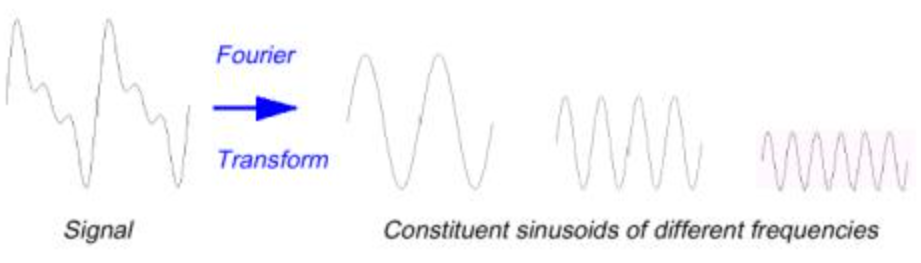
\includegraphics[scale=0.4]{img/wavelet.PNG}
\caption{Wavelet representation}
\label{fig:wavelet}
\end{figure}

A Wavelet is a time-localized wave-like oscillation; an example is shown in Figure \ref{fig:wavelet}. Scale and location are the two most basic features of wavelets. The scale (or dilation) of a wavelet determines how "stretched" or "squished" it is. This attribute has to do with how waves are characterized in terms of frequency. The wavelet's position in time is defined by its location (or space).

Then, the schema of features calculated is as follows. For each lead calculate:

\begin{enumerate}
    \item \textbf{Statistics}: Percentiles (5, 25, 50, 75, 95), mean, standard deviation and variance for the complete signals.
    
    \item Calculate \textbf{coefficients} of \textbf{Discrete Wavelet Transform (DWT)}. DWT gets local frequencies for the signals. The Coefficients are calculated using the function \texttt{wavedec} from the Python’s library \texttt{pywt}.
    
    \item For each \textbf{coefficient} of DWT calculate:
    \begin{itemize}
        \item \textbf{Statistics}: Percentiles (5, 25, 50, 75, 95), mean, standard deviation and variance.
        
        \item \textbf{Shannon’s entropy (same that entropy)}: It’s related to the “amount of information” of a variable. In other words, it measures information of the distribution.
    \end{itemize}
\end{enumerate}


\subsection{Exploratory Data Analysis (EDA)} \label{4eda}

Exploratory Data Analysis refers to the critical process of performing initial investigations on data to identify patterns, spot anomalies, test hypotheses, and check assumptions using summary statistics and graphical representations. It's important to initially comprehend the data before attempting to get as many insights as possible. EDA is all about making sense of data before getting their hands dirty with it. The major steps commonly examined in an EDA are shown in Figure \ref{fig:eda}.

\begin{figure}[H]
\centering
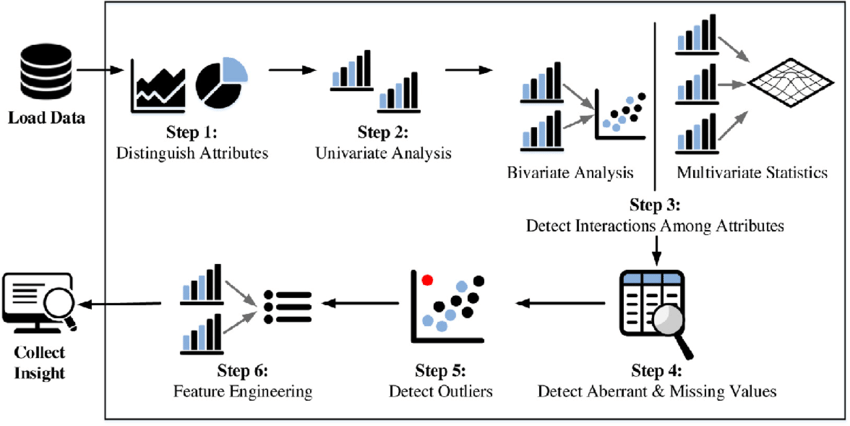
\includegraphics[scale=0.4]{img/EDAschema.PNG}
\caption{Schema of a EDA}
\label{fig:eda}
\end{figure}

\subsection{Unbalanced classes} \label{3unbclass}

One of the most difficult issues when training a model is modeling imbalanced data \cite{smote1}. When dealing with classification problems, the intended class balance is quite important. When a dataset has an uneven distribution of classes, the models attempt to learn only the dominant class, resulting in biased predictions.

One approach for addressing this issue is random sampling. Random resampling can be accomplished in two ways, each with its own set of benefits and drawbacks:

\begin{itemize}
    \item \textbf{Oversampling:} Replicating examples from the minority class.
    \item \textbf{Undersampling:} Deleting examples from the majority class.
\end{itemize}

To put it another way, both oversampling and undersampling include creating bias by selecting more instances from one class than from another. The prior is used to compensate for an imbalance that is already present in the data or that is likely to occur if a perfectly random sample is obtained \cite{smote2}. Because it makes no assumptions about the data, random sampling is a naive strategy. To minimize the data's influence on the Machine Learning algorithm, a fresh adjusted version of the data with a new class distribution is generated.

Random Oversampling and SMOTE were the two oversampling techniques chosen for this project. Synthetic Minority Oversampling Technique is a technique for creating synthetic samples for the minority class. Overcoming the problem of overfitting produced by random oversampling is easier with this method. It focuses on the feature space in order to generate new examples by interpolating between positive occurrences that are near in proximity.

\begin{figure}[H]
\centering
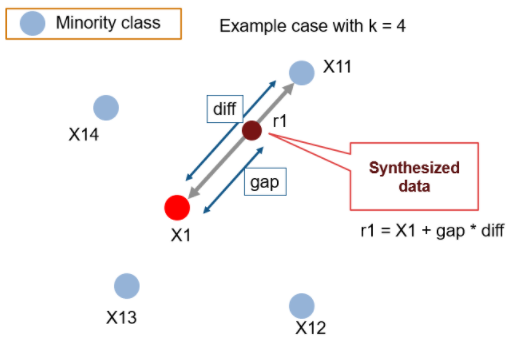
\includegraphics[scale=0.7]{img/SMOTE.PNG}
\caption{SMOTE process illustration}
\label{fig:smoteproc}
\end{figure}

SMOTE uses the k-nearest neighbor technique to create synthetic data. To make them, it follows the instructions below. \cite{smote1}:

\begin{enumerate}
    \item Find the nearest neighbors of the feature vector.
    \item Determine the distance between the two sample sites.
    \item At random, the distance is multiplied by an integer between 0 and 1.
    \item Find a new point on the line segment at the calculated distance.
    \item Rep the procedure for each of the feature vectors that were discovered.
\end{enumerate}

\subsection{Machine Learning Models} \label{3mlmodels}

Classifiers are the models provided in the following sections. These tools were created with the goal of determining which behaviors are more likely to be associated with various arrhythmia patterns. Each of these methods is widely utilized in various data-driven systems, and they have demonstrated useful behavior in a variety of classifying tasks, including ECG classification (\ref{methods_ECG_class}).

The various versions of the dataset were created using Python Notebooks in Google Colab. This section will detail the key models that were tested and evaluated.

\subsubsection{Model 1 - (XGB) XG-Boost algorithm} \label{3model1}

The XG-Boost technique, which has proven to be effective in a variety of classification and regression problems, is the first attempt to classify the ECG signals. The aforementioned algorithm has been used to a variety of sectors, including economics, credit rating, and health-related difficulties. The preceding are reasons to expect that such a strategy will be effective in the field of arrhythmia detection today.

XG-Boost is a decision-tree-based ensemble Machine Learning approach that uses gradient boosting (\cite{xgb1} \cite{xgb2}). When it comes to unstructured data prediction, \textit{Artificial Neural Networks} outperform all other algorithms or frameworks (text, audio, pictures, etc.). However, for small-to-medium tabular data, such as the one utilized in this challenge, \textit{decision tree-based} algorithms are now rated best-in-class.

XG-Boost minimizes a loss function to provide an additive expansion of the objective function, similar to gradient boosting. Because XG-Boost is only interested in decision trees as base classifiers, the complexity of the trees is controlled using a variation of the loss function.

\begin{equation}
L = \sum_{i=1}^{n}{L(y_i,\hat{y_i})}+\sum_{k=1}^{K}{\Theta(p_k)}
\end{equation}
\begin{equation}
\Theta(w)=\gamma Z+\frac{1}{2} \lambda ||w||^2
\end{equation}

\noindent

The number of leaves on the tree is Z, and the leaf output scores are w (\cite{xgb2}). This loss function can be included into the split criterion of decision trees, resulting in a pre-pruning strategy. Trees with a greater $\gamma$ value are easier to understand. The amount of loss reduction gain required to separate an internal node is determined by $\gamma$ (\cite{xgb1}). Shrinkage is a regularization parameter in XG-Boost that decreases the step size in the additive expansion. Finally, other techniques such as tree depth can be utilized to keep the trees from becoming too complex. As a result of lowering tree complexity, the models are trained faster and need less storage space.

\subsubsection{Model 2 - (Catboost) Catboost} \label{3model2}

The second candidate in predicting the arrhythmia type for ECG is the Catboost algorithm. The latter is a decision tree gradient boosting technique. It was created by Yandex (with its final version in 2017) researchers and engineers and is used by Yandex and other firms such as CERN, Cloudflare, and Careem taxi for search, recommendation systems, personal assistant, self-driving cars, weather prediction, and many other activities. Anyone can use it because it is open-source.

\begin{figure}[H]
\centering
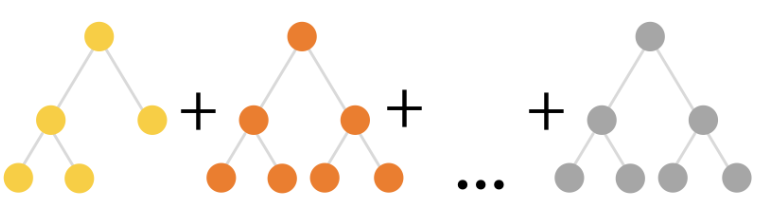
\includegraphics[scale=0.6]{img/catboost.PNG}
\caption{Catboost (decision trees) illustration}
\label{fig:catboost}
\end{figure}

The implementation of ordered boosting \cite{catboost}, a permutation-driven alternative to the conventional approach, and a novel technique for processing category characteristics are two key algorithmic innovations offered in CatBoost. Both strategies were developed in order to combat a prediction shift induced by a specific type of target leakage found in all current gradient boosting algorithm implementations.

\subsubsection{Model 3 - (DNN) Deep Neural Networks} \label{3model3}

A Deep Neural Network is another method for predicting ECG diagnosis. A DNN is a set of algorithms that attempts to recognize relationships in a batch of data by mimicking how the human brain functions.

In this context, deep neural networks refer to organic or artificial systems of neurons (\cite{ann1}). Deep neural networks can adapt to changing input and produce the best possible result without requiring the output criteria to be modified because they can adapt to changing input. Neural networks, an artificial intelligence-based concept, are swiftly gaining popularity in the development of trading systems.

Neural networks aid in time-series forecasting, algorithmic trading, securities classification, credit risk modeling, and the generation of proprietary indicators and price derivatives in the financial world (\cite{ann2} \cite{ann3}). The deep neural network of the human brain is akin to a neural network. A "neuron" in a deep neural network is a mathematical function that collects and categorizes data according to a set of rules. The network closely resembles curve fitting and regression analysis, two statistical methods.

\begin{figure}[h!]
\centering
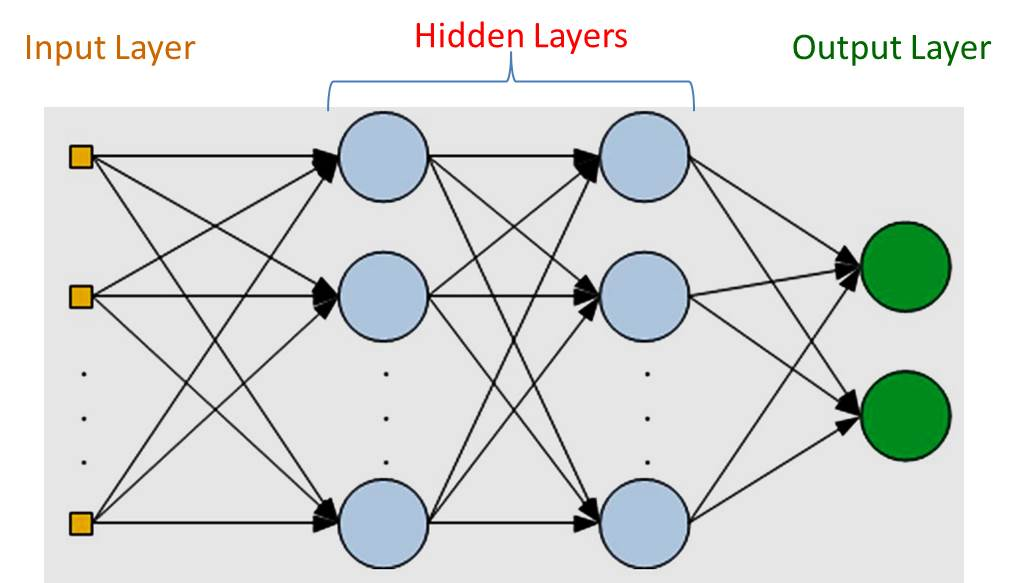
\includegraphics[scale=0.6]{img/Multilayer-Perceptron.jpg}
\caption{Deep Neural Network (Multi-layer Perceptron) schema}
\label{fig:mlp}
\end{figure}

Perceptrons are grouped in interconnected layers in a multi-layered perceptron (MLP) \cite{ann3}, as indicated in Figure \ref{fig:mlp} . The input layer is responsible for collecting input patterns. In the output layer, input patterns can be mapped to classifications or output signals. Hidden layers fine-tune the input weightings until the neural network's margin of error is as little as possible. Hidden layers are supposed to deduce salient elements from input data that have the ability to predict outcomes. This is how feature extraction works, and it's similar to how statistical methods such as principal component analysis function (\cite{ann3}).

\subsubsection{Model 4 - (LSTM) Long-Short Term Memory} \label{3model4}

Long short-term memory networks, are a type of Deep Learning network. It's a class of recurrent neural networks (RNNs) that can learn long-term dependencies, which is useful for solving sequence prediction issues. Apart from single data points like photos, LSTM has feedback connections, which means it can process the complete sequence of data.

\begin{figure}[h!]
\centering
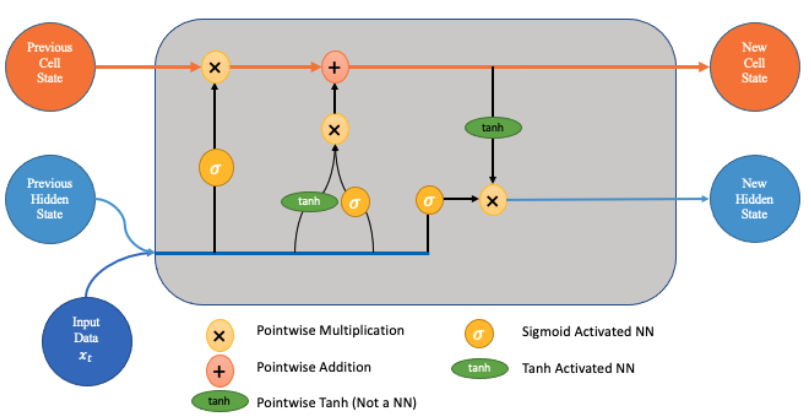
\includegraphics[scale=0.5]{img/lstm.png}
\caption{LSTM general schema}
\label{fig:lstm}
\end{figure}

An LSTM model's primary role is played by a memory cell called a 'cell state,' which maintains its state across time. The horizontal line that runs through the top of the diagram below represents the cell state. It can be compared to a conveyor belt on which data just passes, unmodified \cite{lstm}.

\subsection{Metrics} \label{3metrics}

It is vital to create metrics that will assist in determining whether a model is better than others in order to determine whether it is better than others. There are explanations for each of the metrics used in the following sections.

\subsubsection{Confusion Matrix} \label{4confmatrix}

A confusion matrix, like the one shown in table \ref{table:confmatr}, demonstrates how well a classification model works on test data for which the true values are known (\cite{metrics2}). The confusion matrix is simple in itself, but the related nomenclature can be confusing. In the following examples, I've created a hypothetical target variable called "Diagnose A" with the values "Yes" (if the recording belongs to that diagnose) and "No" (if the recording does not belong to that diagnose).


\begin{table}[H]
\centering
\begin{tabular}{ |p{4cm}||p{4cm}||p{4cm}|  }
 \hline
 \multicolumn{3}{|c|}{\textbf{Actual Class}} \\
 \hline
 \textbf{Predicted Class}  & Diagnose A - YES = 1 & Diagnose A - NO = 0\\
 \hline
 Diagnose A - YES = 1 & True Positives (\textbf{TP})  & False Positives (\textbf{FP}) \\
 Diagnose A - NO = 0 & False Negatives (\textbf{FN})  & True Negatives (\textbf{TN}) \\
 \hline
\end{tabular}
\caption{Confusion Matrix representation}
\label{table:confmatr}
\end{table}

Here is an explanation for each of the matrix's elements to understand the preceding terminology (\cite{metrics2} \cite{metrics1}).

\begin{itemize}
    \item \textit{True negatives (TN):} The model predicted they wouldn't have the diagnose A, and they don't.
    \item \textit{True positives (TP):} These are examples when the model predicted yes (the recording has the diagnose A), and they actually don't.
    \item \textit{False positives (FP):} The model projected that they would have the diagnose A, but they don't. (This is also referred to as a "Type I error.")
    \item \textit{False negatives (FN):} The model anticipated that they would not have diagnose A, yet they do. (This is often referred to as a "Type II error.")
\end{itemize}

\subsubsection{Accuracy} \label{4accuracy}

\begin{equation}
    Accuracy = \frac{TP+TN}{TP+FP+FN+TN}
\end{equation}

The most basic performance metric is accuracy, which is defined as the proportion of correctly predicted observations to all observations. If a model is correct, one would assume it is the best. Yes, accuracy is a relevant measure when the datasets are symmetric and the number of false positives and false negatives is about equal.

Imagining the case when the training set contains 98 percent samples of class A and $2\%$ samples of class B, for example. The model may thus easily attain a $98\%$ training accuracy by simply guessing every training sample that belongs to class A. When the same model is tested on a test set that contains $60\%$ class A samples and $40\%$ class B samples, the test accuracy reduces to $60\%$. As a result, classification accuracy is poor, but it gives the image of great accuracy.

Then, when the cost of misclassification of minor class samples becomes significant, (\cite{metrics1}) the true issue appears. The cost of failing to diagnose, for example, a sick person's ailment is significantly greater than the expense of submitting a healthy person to additional tests when dealing with a rare but lethal disorder.

\subsubsection{Precision} \label{4precision}
\begin{equation}
    Precision = \frac{TP}{TP+FP}
\end{equation}

Precision \cite{metrics2} is the ratio of accurately predicted positive observations to total expected positive observations. This measure answers the question of how many of the drivers who were identified as drowsy actually drove. Precision is linked to a low false-positive rate.

Precision is a good statistic to employ when the costs of False Positive are high. Take, for example, the identification of email spam. In email spam detection, a false positive happens when an email that is not spam (actual negative) is wrongly identified as spam (predicted spam). If the precision of the spam detection model is low, the email user may miss important emails.

\subsubsection{Recall} \label{4recall}
\begin{equation}
    Recall = \frac{TP}{TP+FN}
\end{equation}

Recall \cite{metrics2} is the ratio of successfully predicted positive observations to all observations in the actual class. It's meant to answer the question of how many drivers who actually slept were labeled as such.

In the case of identifying sick patients, for example, if a sick patient (Actual Positive) conducts the test and is predicted to be healthy (Predicted Negative). The cost of False Negative will be quite high if the condition is infectious.

\subsubsection{F1 Score} \label{4F1}
\begin{equation}
    F1 Score = \frac{2*(Recall * Precision)}{(Recall + Precision)}
\end{equation}

The F1-Score is the weighted average of Precision and Recall. As a result, both false positives and false negatives are taken into account in this score. F1 is often more valuable than accuracy, despite the fact that it is less intuitive (\cite{metrics1} \cite{metrics2}). This is especially true if the class distribution is unequal. When the costs of false positives and false negatives are equal, accuracy works well. If the cost of false positives and false negatives differs significantly, it is best to evaluate both Precision and Recall.

\subsubsection{Overall index} \label{4overallindex}

As a final metrics, I introduced the use of the mean value of Accuracy, Precision, Recall and F1-Score. With the latter, it is possible to check with only one metric the overall behaviour of the classifiers.

% \subsection{Fine tuning hyper parameters} \label{3finetuning}

% Models for machine learning are made up of two sorts of parameters:

% \begin{itemize}
%     \item - \textbf{Hyper parameters:} Those are all the parameters that the user can specify freely before beginning training (e.g. number of estimators in XG-Boost).
%     \item - \textbf{Model parameters:} Those are learned during model training instead (e.g. weights in Neural Networks).
% \end{itemize}

% The model parameters are learned during training and define how to use input data to produce the desired output. Hyperparameters, on the other hand, govern how the model is structured. Tuning Machine Learning models is an example of an optimization problem. There are a set of hyperparameters, and the objective is to determine the best combination of their values to find the minimum (for example, loss) or maximum (for example, accuracy) of a function. 

% This is especially significant when evaluating the performance of multiple Machine Learning models on a dataset. Comparing an XG-Boost model with the best hyperparameters against a Neural Network model that has not been optimized would be unfair.

% \begin{figure}[H]
% \centering
% 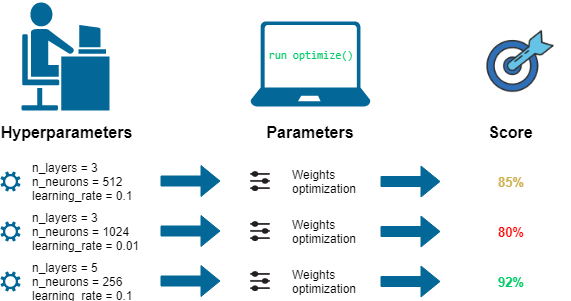
\includegraphics[scale=0.5]{finetuning.png}
% \caption{Example hyper parameters fine tuning }
% \label{fig:finetuning}
% \end{figure}


% Along with this thesis, there are two main approaches used to find the optimal hyper parameters for the selected methods: Grid search and Random Search.

% \subsubsection{Grid Search} \label{31gridsearch}

% One can put up a grid of hyperparameters in Grid Search and train/test the model on all the potential combinations. To determine the parameters to utilize in Grid Search, one may now look at several possible ranges and create a grid-based on them to see if a better combination can be found. The scikit-learn \textit{GridSearchCV()} function can be used to implement Grid Search in Python.

% \subsubsection{Random Search} \label{31randomsearch}

% In Random Search, a grid of hyperparameters is created, and the model is trained/tested using only a random mix of these hyperparameters. In addition, Cross-Validation on the training set is an option. When doing Machine Learning tasks, the dataset is usually divided into training and test sets. This is done so that the model may be tested after it has been trained (in this way, it is possible to check its performances when working with unseen data). To ensure that our model is not overfitting the data, we divide the training set into K other divisions using Cross-Validation.


\section{Federated learning (FL) fundamentals} \label{4fedlea}

\subsection{Definition}
Federated learning (FL) is a machine learning technique for training machine learning models cooperatively on several devices or local servers in a decentralized way, preserving data privacy and data ownership for the device/server owner \cite{fl8}. FL is extremely advantageous for highly decentralized healthcare data, especially with the growing prevalence of IoT devices for continuously capturing data and monitoring health.


\begin{figure}[H]
\centering
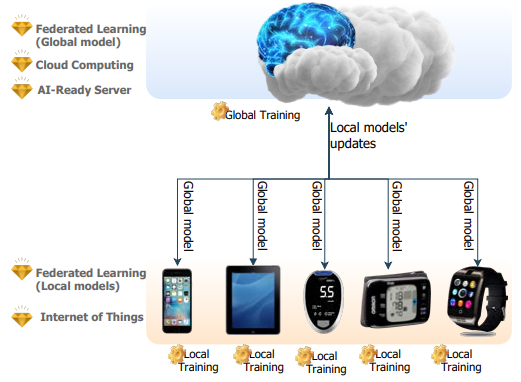
\includegraphics[scale=0.6]{img/fl_overview.png}
\caption{FL framework Overview}
\label{fig:fl_overview}
\end{figure}

Figure \ref{fig:fl_overview} depicts a high-level view of the framework and how the technologies will interact together. The IoT devices will collect data from users and train a local deep learning model that is a copy of a global model that was previously received. Following the completion of the local training phase, the models will collaborate to train a global model utilizing their updates rather than the raw data provided by the users. These model updates indicate changes in the weights of the models during the training process and do not reflect any private or personal information about the users.

All participating models will send updates to a cloud server, where they will be compiled and used to train the global model \cite{fl2} \cite{fl3}. Each device will receive a new copy of the updated global model once the global model training procedure is completed. As a result, the models will be trained and updated on a regular basis without sharing any personal information. As a result, the framework will support an IoT-based decentralized architecture in which models are spread among IoT devices without the need for a centralized server to operate the model and serve users. It will also protect users' privacy by processing and analyzing their data on IoT devices without disclosing it.

\subsection{FL types}

FL is divided into five categories \cite{fl26_types} based on data partitioning, machine learning models (ML Models), privacy mechanisms, communication architecture, and federation scale.

\subsubsection{Data Partitioning}

The datasets of various clients share the same properties in \textbf{Horizontal data partitioning} \cite{fl25}, however there is limited sample space intersection. All FL architectures use horizontal partitioning the most. Aggregation at the server is made easier by the fact that a standard model can be used for all clients; FedAvg is typically used for aggregation. A dataset containing ONLY breast cancer patients from a specific hospital would be a simple to comprehend example. 

\begin{figure}[H]
\centering
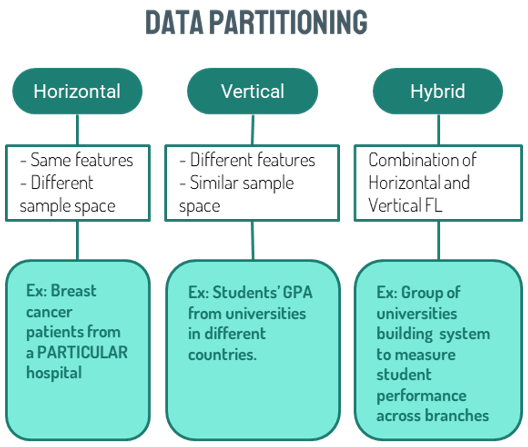
\includegraphics[scale=0.5]{img/fl_data_partition.png}
\caption{Data partition-based FL types}
\label{fig:fl_data_partition}
\end{figure}

When clients are exposed to distinct feature spaces but the same or similar sample space, \textbf{Vertical Data Partitioning} comes into play. Entity alignment algorithms are utilized to find overlapping samples among the client data, and this overlapped data is used for training \cite{fl26_types}. A dataset of students' GPAs obtained from institutions across the globe is a nice example. The feature space, which includes the grading scale and evaluation measure, is distinct.

Horizontal and vertical data partitioning are combined in \textbf{Hybrid Data Partitioning}. A set of universities intending to develop a FL System to assess student achievement across branches is an easy to comprehend case for hybrid partitioning.

\subsubsection{ML models}

The issue statement and dataset are frequently used to determine the machine learning models to use \cite{fl26_types}. One of the most widely used models is neural networks (NN). Apart from NNs, decision trees are also used, as they are highly efficient and simple to understand. Models can be \textbf{homogeneous} or \textbf{heterogeneous} in a FL system. 

\begin{figure}[H]
\centering
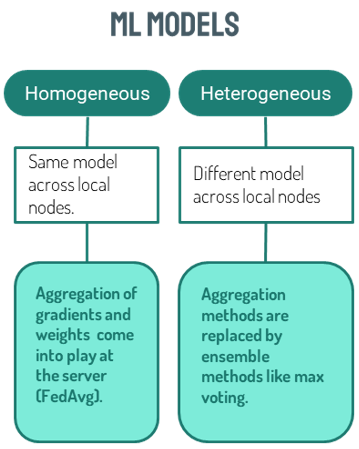
\includegraphics[scale=0.5]{img/fl_mlmodels.png}
\caption{ML models-based FL types}
\label{fig:fl_mlmodels}
\end{figure}

In the case of the former, all clients use the same model, while the server uses gradient aggregation. In the latter instance, however, there is no possibility of aggregating because each client has a unique model. Aggregation methods are substituted with ensemble methods like max voting at the server in the case of heterogeneous models \cite{fl26_types}.

\subsubsection{Privacy Mechanisms}

The most controversial part of FL is how it deals with privacy. The main concept is to prevent client information from leaking out. The server may decipher the data of clients without encryption by applying learning gradients. As a result, it's critical to hide the gradients. Differential privacy and cryptographic approaches are commonly used to address privacy concerns in FL systems.

\begin{figure}[H]
\centering
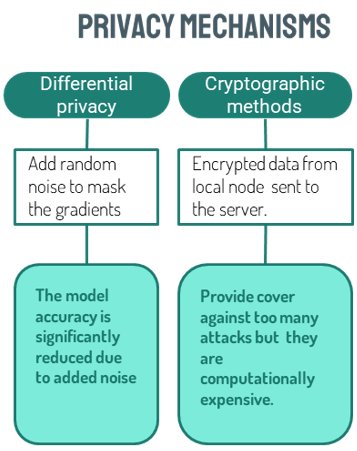
\includegraphics[scale=0.5]{img/fl_privacy_methods.png}
\caption{Privacy Mechanisms-based FL types}
\label{fig:fl_privacy_methods}
\end{figure}

\textbf{Differential privacy} is a technique for hiding gradients by adding random noise to data or model parameters. Due to the extra noise, this strategy has a considerable negative in terms of model accuracy.

In FL systems, \textbf{cryptographic approaches} such as homomorphic encryption and safe multi-party computation are commonly used. The process is straightforward: clients send encrypted data to the server, the server processes the data, and then the encrypted output is decrypted to obtain the final result. Despite the fact that these methods provide protection against a wide range of threats, they are computationally intensive.

\subsubsection{Architecture}

There are two types of FL system architecture: centralized and decentralized. Both types of architecture work in the same way; the only difference is in client-server communication. We have a second model that acts as a server in a \textbf{centralized architecture}, and all parameter updates are done in this global model. 

\begin{figure}[H]
\centering
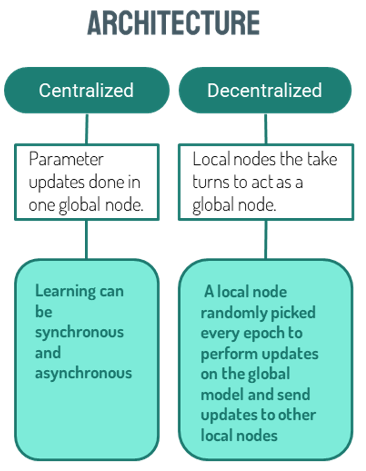
\includegraphics[scale=0.5]{img/fl_architecture.png}
\caption{Architecture-based FL types}
\label{fig:fl_architecture}
\end{figure}


In a \textbf{decentralized design}, on the other hand, clients take turns acting as servers. Every epoch, a client is chosen at random to make global model changes and send the global model to other clients.

\subsubsection{Scale of Federation}

The scale of federation can be divided into two types: cross-silo and cross-device. To grasp the distinction between the two, relate cross-silo with organizations and cross-devices with mobiles. When using \textbf{cross-silo}, the number of clients is usually minimal, but they have a lot of computing power. 

\begin{figure}[H]
\centering
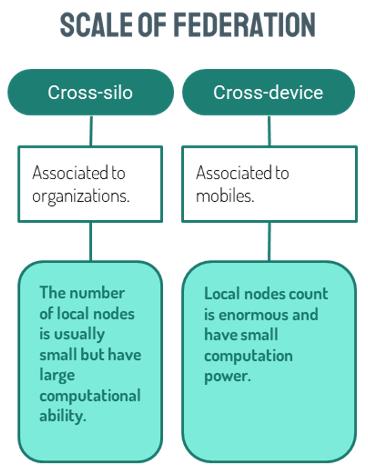
\includegraphics[scale=0.5]{img/fl_scale.png}
\caption{Scale of federation-based FL types}
\label{fig:fl_scale}
\end{figure}

Regarding \textbf{cross-device}, the number of clients is enormous, but their computing power is limited. Another consideration is reliability: while we can rely on organizations (cross-silo) to be ready to train at all times, this is not the case with mobile phones (cross-devices). There's a chance that a bad network will make the gadget unavailable.

\subsection{Advantages and disadvantages}

FL has a lot of advantages over traditional, centralized systems \cite{fl27_adv_disadv}. Some of the most remarkable The upper hands of FL are:

\begin{itemize}
    \item \textbf{Data security}: Keeping the training dataset on the devices eliminates the need for a data pool for the model.
    \item \textbf{Data diversity}: Companies may be unable to merge datasets from diverse sources due to challenges other than data security, such as network unavailability in edge devices. Federated learning makes it easier to access diverse data, even when data sources can only interact at particular periods.
    \item \textbf{Continuous learning in real time}: Models are continuously enhanced utilizing client input, eliminating the requirement to aggregate data for continuous learning.
    \item \textbf{Technology efficiency}: Because federated learning models do not require a single complex central server to evaluate data, this technique requires less complex hardware.
\end{itemize}

On the other hand, FL need to deal with some relevant challenges. The most common are:

\begin{itemize}
    \item \textbf{Investment requirements}: FL models may necessitate frequent communication between nodes, which may necessitate an investment. This means that high bandwidth and storage capacity are among the system requirements.
    
    \item \textbf{Data Privacy}: In FL, data is not collected on a single entity/server; instead, numerous devices are used to collect and analyze data. Even though only models, not raw data, are transferred to the central server, models can be reverse engineered to identify client data, thereby increasing the attack surface. Differential privacy, secure multiparty computation, and homomorphic encryption are examples of privacy-enhancing technologies that can be utilized to improve the data privacy capabilities of federated learning.
    
    \item \textbf{Performance limitations}: In FL, models from several devices are combined to create a superior model. Device-specific factors may hinder the generalization of models from some devices, lowering the accuracy of the model's next generation. Researchers investigated scenarios in which one of the federation's members could use secret backdoors in the joint global model to intentionally attack others.
\end{itemize}

\subsection{Proposed approaches} \label{proposed_approaches}

After understanding the theory and characteristics behind the FL techniques I decided to test two different approaches using the PhysioNet 2020 datasets.

The first approach can be visualized in Figure \ref{fig:fl_approach1}. It is going to be called the Independent and Identically distributed \textbf{(IID) approach}. 

\begin{figure}[H]
\centering
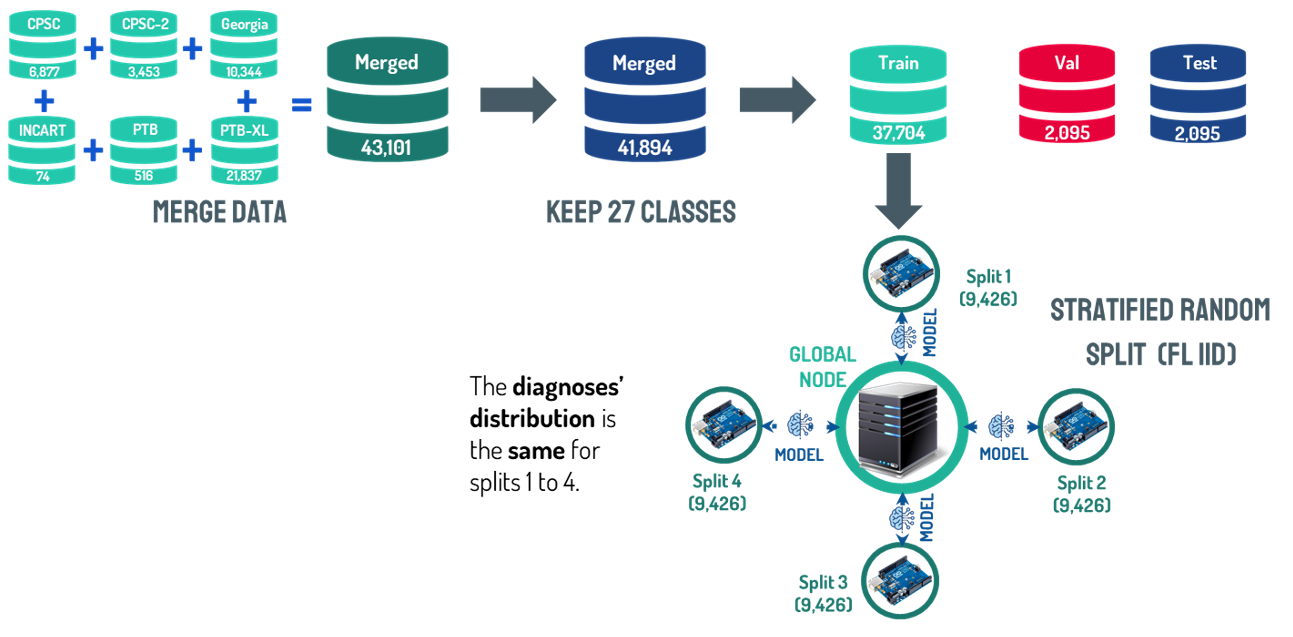
\includegraphics[scale=0.4]{img/fl_approach1.png}
\caption{Approach 1: IDD approach}
\label{fig:fl_approach1}
\end{figure}

In the IID approach, I took the 6 databases (more information here xx) and appended them all in a single dataset with 43,101 recordings. After, using the analysis explained in xx, I ended up with 41,894 (filtering out the non-representative classes). Afterwords, I randomly split the data to get train, validation and test datasets. Afterwords, to get the IID splits I performed a Stratified random split, dividing the whole train data in 4 parts. In that way, the distribution of the labels (diagnoses) is the same for each partition.

The second (and more real) approach was called the \textbf{(Non-IID) approach}. It's structure is explained in figure \ref{fig:fl_approach2}.

\begin{figure}[H]
\centering
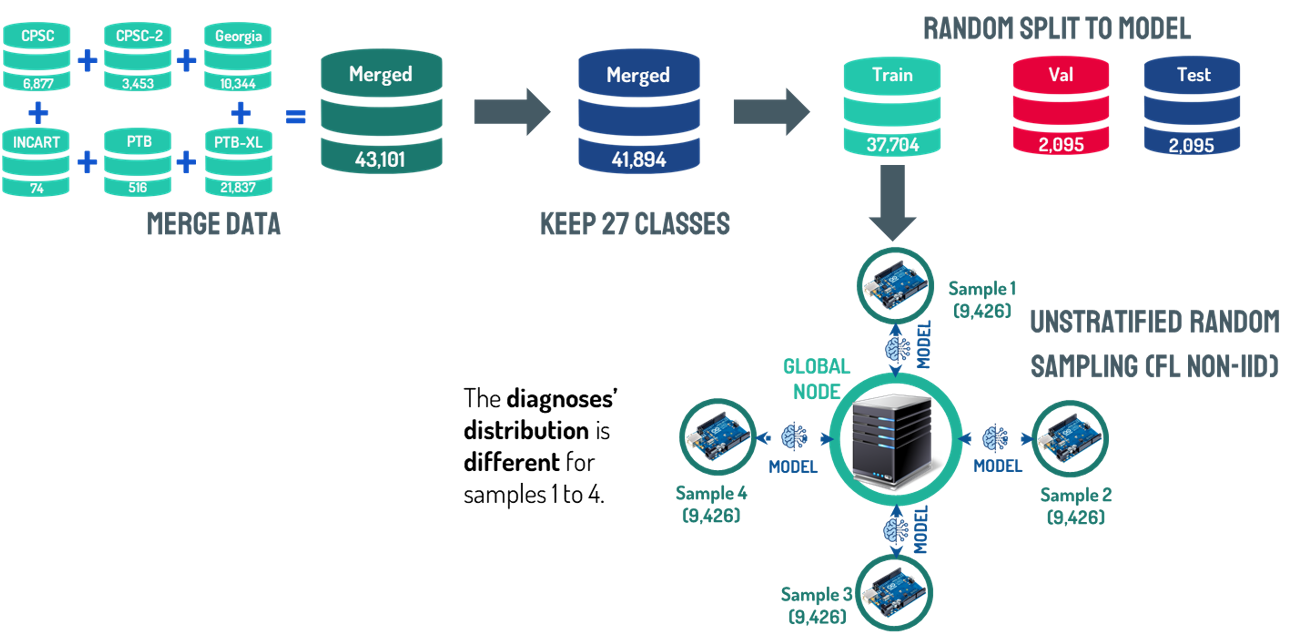
\includegraphics[scale=0.4]{img/fl_approach2.png}
\caption{Approach 2: Non-IID approach}
\label{fig:fl_approach2}
\end{figure}

In the Non-IID approach, I combined all six datasets (additional information here xx) into a single dataset including 43,101 recordings. I came up with 41,894 after utilizing the methodology described in xx (filtering out the non-representative classes). After that, I divided the data into train, validation, and test datasets at random. Later, I used an Unstratified random sampling (with replacement) method to acquire four separate samples from the original data. As a result, each sample has a varied distribution of labels (diagnoses).



























